\documentclass[../main.tex]{subfiles}

\begin{document}

\section{Lecture 11 -- Structured Prediction}

\begin{remark}
    \begin{center}
        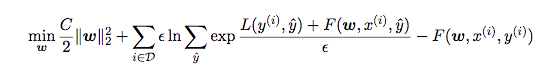
\includegraphics[width=\textwidth,height=\textheight,keepaspectratio]{lecture9_general_loss}
    \end{center}

    The general loss function above can be interpolated or specified to be obtain
    either the multiclass logistic loss function or the multiclass svm loss function.

    To obtain the multiclass logistic loss function, set $\e = 1$ and $L = 0$.

    \begin{align*}
        \sum_{i \in D}^{} \log \left( \sum_{\hat{y}}^{}\exp{\left( \hat{y}w^T\phi(x) - y_{i}w^T\phi(x) \right)} \right) \\
        = - \sum_{i \in D}^{}\log \frac{1}{\left( \sum_{\hat{y}}^{}\exp{\left( \hat{y}w^T\phi(x) - y_{i}w^T\phi(x) \right)} \right)} \\
        \intertext{Now do some additional manipulation}
        = - \sum_{i \in D}^{}\log \frac{\exp{(y_{i}w^T\phi(x))}}{\left( \sum_{\hat{y}}^{}\exp{\left( \frac{\hat{y}w^T\phi(x)}{1} \right)} \right)} \\
    \end{align*}

    If we set $\e \to 0$ and $L = 1$, then we recover the SVM multiclass classification function.

\end{remark}

\begin{definition}
    A prediction problem is to find $y^{\ast}$ where

    \[
        y^{\ast} = \arg \max_{\hat{y}} F(w,x,\hat{y})
    \]

    where $y^{\ast}$ is some vector of values.
\end{definition}

\begin{remark}
    A first temptation is to frame every such maximizatin problem as a maximization
    over each of its subcomponents.

    That is, maximize

    \[
        \sum_{y_d \in y^{\ast}}^{}F_d(w,x,y_d)
    \]

    but doing so would ignore that, oftentimes, there is structural knowledge that
    aids in the learning problem. That is, oftentimes, we gain information by
    looking at several components collectively. 
\end{remark}

\begin{example}
    If we were given the four letters to the far left and classified them by
    looking exclusively at each letter, we might think that we should predict
    Q V I Z. In reality, however, if we look at the letters holistically,
    we can predict QUIZ.

    \begin{center}
        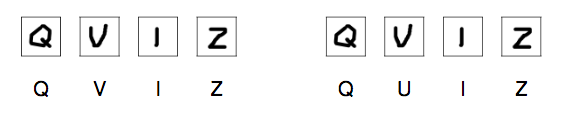
\includegraphics[width=\textwidth,height=\textheight,keepaspectratio]{lecture9_quiz}
    \end{center}

    At one extreme, we can perform a holistic evaluation by solving
    \[
        \max_{D \in A^4}F_D(w,x,y_D) 
    \]

    where $\abs{A}$ is the set of letters. There are far too many possibilities here.
    At the other extreme, we can perform discretization by solving

    \[
        \sum_{i=1}^{n}\max_{d \in A}F_d(w,x_i,y_d) 
    \]

    This does not take into account correlations between letters.
\end{example}

\begin{remark}
    We can perform structural prediction over pairs of attributes, for this reason:
    \begin{center}
        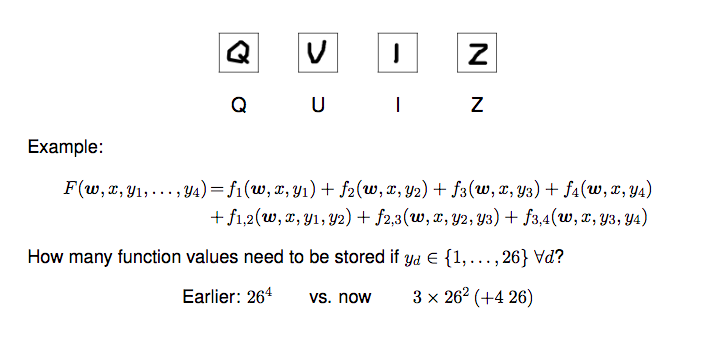
\includegraphics[width=\textwidth,height=\textheight,keepaspectratio]{lecture9_quiz_reex}
    \end{center}

    This gives us $3 \times 26^2 + 4(26)$ labelings that we consider.
    This can be visualized as a diagram:

    \begin{center}
        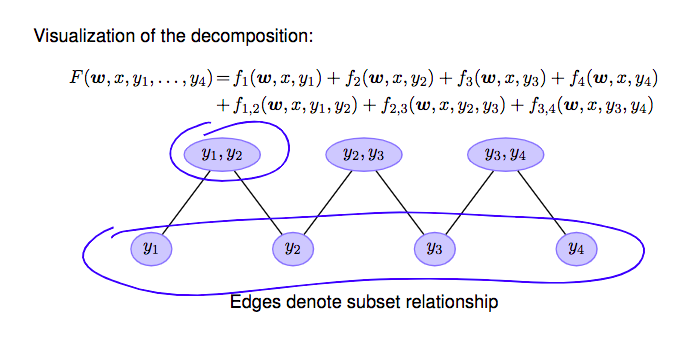
\includegraphics[width=\textwidth,height=\textheight,keepaspectratio]{lecture9_quiz_vis}
    \end{center}


\end{remark}

\begin{remark}
    There are a few algorithms one can employ to perform this search: One is Exhaustive Search:

    \begin{center}
        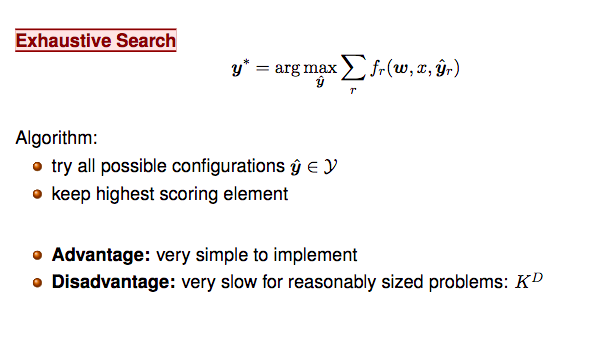
\includegraphics[width=\textwidth,height=\textheight,keepaspectratio]{lecture9_exhaustive_search}
    \end{center}

    Another is dynamic programming:

    \begin{center}
        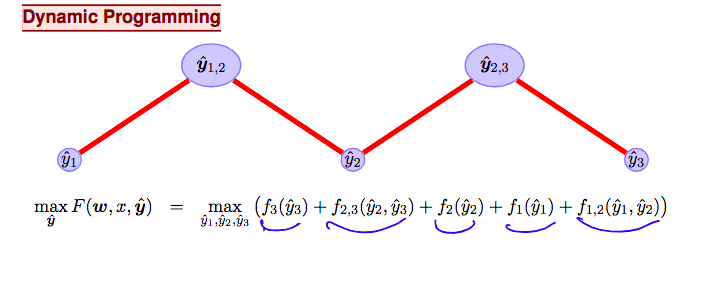
\includegraphics[width=\textwidth,height=\textheight,keepaspectratio]{lecture9_dp}
    \end{center}

    Recall that a problem admits a solution via dynamic programming if it satisfies
    two criterion: a problem can be decomposed into subproblems, and these subproblems
    overlap; a problem has the principle of optimality which is that the optimal
    solution to a problem is a function of the optimal solution of some of its subproblems. \\

    Above, we see that if we define one problem $P$ to be maximization of the objective
    function over all $5$ nodes, then this problem has a subproblem $S$: maximization
    over all nodes but $\hat{y}_3$. After $S$ is solved, solving
    $P$ then requires maximizing over the nodes involving $\hat{y}_3$. Whence,
    this problem has the principle of optimality and admits a DP solution.

    This is formalized by splitting the application of $\max$ as below.

    \begin{center}
        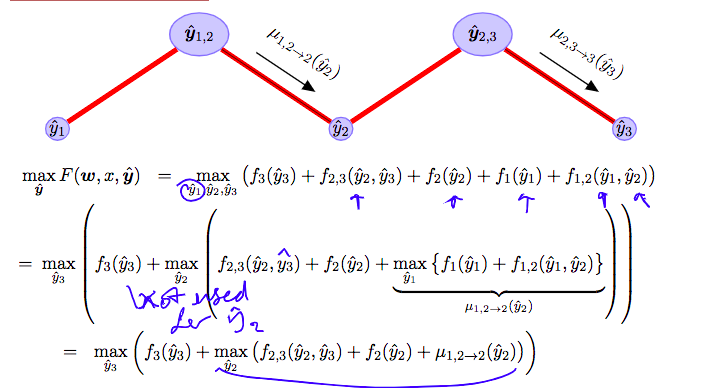
\includegraphics[width=\textwidth,height=\textheight,keepaspectratio]{lecture9_dp_formal}
    \end{center}

    This is colloquially called ``message'' passing, because we pass the optimal solution
    obtained from maximizing $\hat{y}_1$ and $\hat{y}_{1,2}$ to a problem maximizing
    over $\hat{y}_2$ and then pass that problem to a problem maximizing over $\hat{y}_3$.

    The summary of DP is as follows. Note that $K$ is the amount of values that
    any one dimension of $y_D$ can take on. Thus, if there is a tree of $D$ nodes
    that each involve maximization over a pair of dimensions in $y_D$, then there
    are $D \cdot K^2$ values that we must work through.
    \begin{center}
        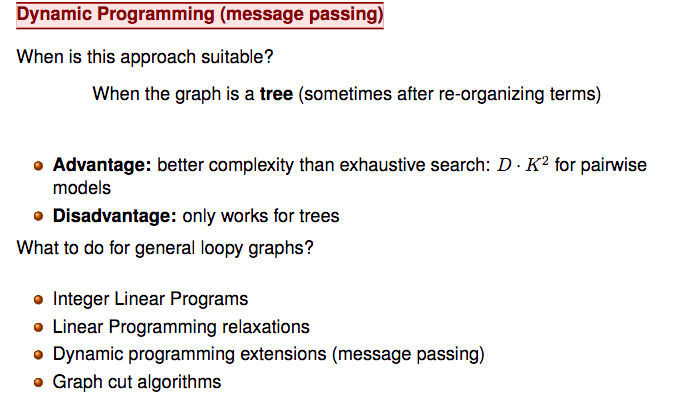
\includegraphics[width=\textwidth,height=\textheight,keepaspectratio]{lecture9_dp_summary}
    \end{center}
\end{remark}<++>
\end{document}
